% Rankings are META-DERIVED, not independently judged agronomic safety.
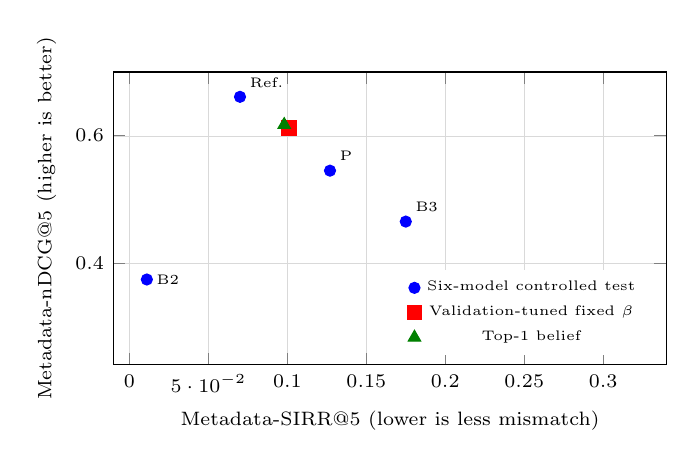
\begin{tikzpicture}
\begin{axis}[
  width=8.6cm, height=5.3cm,
  xlabel={Metadata-SIRR@5 (lower is less mismatch)},
  ylabel={Metadata-nDCG@5 (higher is better)},
  xmin=-0.01, xmax=0.34, ymin=0.24, ymax=0.70,
  tick label style={font=\scriptsize},
  label style={font=\scriptsize},
  grid=major, grid style={line width=0.1pt, draw=black!15},
  legend style={at={(0.97,0.03)},anchor=south east,font=\tiny,draw=none},
]
\addplot[only marks,mark=*,mark size=2pt,blue] coordinates {
(0.218,0.283) (0.301,0.343) (0.011,0.374) (0.175,0.465)
(0.127,0.545) (0.070,0.661)};
\addlegendentry{Six-model controlled test}
\addplot[only marks,mark=square*,mark size=2.6pt,red] coordinates {(0.101,0.612)};
\addlegendentry{Validation-tuned fixed $\beta$}
\addplot[only marks,mark=triangle*,mark size=2.6pt,green!50!black] coordinates {(0.098,0.617)};
\addlegendentry{Top-1 belief}
\node[font=\tiny,anchor=south west] at (axis cs:0.218,0.283) {B0};
\node[font=\tiny,anchor=south east] at (axis cs:0.301,0.343) {B1};
\node[font=\tiny,anchor=west] at (axis cs:0.011,0.374) {B2};
\node[font=\tiny,anchor=south west] at (axis cs:0.175,0.465) {B3};
\node[font=\tiny,anchor=south west] at (axis cs:0.127,0.545) {P};
\node[font=\tiny,anchor=south west] at (axis cs:0.070,0.661) {Ref.};
\end{axis}
\end{tikzpicture}
